\documentclass[1p]{elsarticle_modified}
%\bibliographystyle{elsarticle-num}

%\usepackage[colorlinks]{hyperref}
%\usepackage{abbrmath_seonhwa} %\Abb, \Ascr, \Acal ,\Abf, \Afrak
\usepackage{amsfonts}
\usepackage{amssymb}
\usepackage{amsmath}
\usepackage{amsthm}
\usepackage{scalefnt}
\usepackage{amsbsy}
\usepackage{kotex}
\usepackage{caption}
\usepackage{subfig}
\usepackage{color}
\usepackage{graphicx}
\usepackage{xcolor} %% white, black, red, green, blue, cyan, magenta, yellow
\usepackage{float}
\usepackage{setspace}
\usepackage{hyperref}

\usepackage{tikz}
\usetikzlibrary{arrows}

\usepackage{multirow}
\usepackage{array} % fixed length table
\usepackage{hhline}

%%%%%%%%%%%%%%%%%%%%%
\makeatletter
\renewcommand*\env@matrix[1][\arraystretch]{%
	\edef\arraystretch{#1}%
	\hskip -\arraycolsep
	\let\@ifnextchar\new@ifnextchar
	\array{*\c@MaxMatrixCols c}}
\makeatother %https://tex.stackexchange.com/questions/14071/how-can-i-increase-the-line-spacing-in-a-matrix
%%%%%%%%%%%%%%%

\usepackage[normalem]{ulem}

\newcommand{\msout}[1]{\ifmmode\text{\sout{\ensuremath{#1}}}\else\sout{#1}\fi}
%SOURCE: \msout is \stkout macro in https://tex.stackexchange.com/questions/20609/strikeout-in-math-mode

\newcommand{\cancel}[1]{
	\ifmmode
	{\color{red}\msout{#1}}
	\else
	{\color{red}\sout{#1}}
	\fi
}

\newcommand{\add}[1]{
	{\color{blue}\uwave{#1}}
}

\newcommand{\replace}[2]{
	\ifmmode
	{\color{red}\msout{#1}}{\color{blue}\uwave{#2}}
	\else
	{\color{red}\sout{#1}}{\color{blue}\uwave{#2}}
	\fi
}

\newcommand{\Sol}{\mathcal{S}} %segment
\newcommand{\D}{D} %diagram
\newcommand{\A}{\mathcal{A}} %arc


%%%%%%%%%%%%%%%%%%%%%%%%%%%%%5 test

\def\sl{\operatorname{\textup{SL}}(2,\Cbb)}
\def\psl{\operatorname{\textup{PSL}}(2,\Cbb)}
\def\quan{\mkern 1mu \triangleright \mkern 1mu}

\theoremstyle{definition}
\newtheorem{thm}{Theorem}[section]
\newtheorem{prop}[thm]{Proposition}
\newtheorem{lem}[thm]{Lemma}
\newtheorem{ques}[thm]{Question}
\newtheorem{cor}[thm]{Corollary}
\newtheorem{defn}[thm]{Definition}
\newtheorem{exam}[thm]{Example}
\newtheorem{rmk}[thm]{Remark}
\newtheorem{alg}[thm]{Algorithm}

\newcommand{\I}{\sqrt{-1}}
\begin{document}

%\begin{frontmatter}
%
%\title{Boundary parabolic representations of knots up to 8 crossings}
%
%%% Group authors per affiliation:
%\author{Yunhi Cho} 
%\address{Department of Mathematics, University of Seoul, Seoul, Korea}
%\ead{yhcho@uos.ac.kr}
%
%
%\author{Seonhwa Kim} %\fnref{s_kim}}
%\address{Center for Geometry and Physics, Institute for Basic Science, Pohang, 37673, Korea}
%\ead{ryeona17@ibs.re.kr}
%
%\author{Hyuk Kim}
%\address{Department of Mathematical Sciences, Seoul National University, Seoul 08826, Korea}
%\ead{hyukkim@snu.ac.kr}
%
%\author{Seokbeom Yoon}
%\address{Department of Mathematical Sciences, Seoul National University, Seoul, 08826,  Korea}
%\ead{sbyoon15@snu.ac.kr}
%
%\begin{abstract}
%We find all boundary parabolic representation of knots up to 8 crossings.
%
%\end{abstract}
%\begin{keyword}
%    \MSC[2010] 57M25 
%\end{keyword}
%
%\end{frontmatter}

%\linenumbers
%\tableofcontents
%
\newcommand\colored[1]{\textcolor{white}{\rule[-0.35ex]{0.8em}{1.4ex}}\kern-0.8em\color{red} #1}%
%\newcommand\colored[1]{\textcolor{white}{ #1}\kern-2.17ex	\textcolor{white}{ #1}\kern-1.81ex	\textcolor{white}{ #1}\kern-2.15ex\color{red}#1	}

{\Large $\underline{11a_{333}~(K11a_{333})}$}

\setlength{\tabcolsep}{10pt}
\renewcommand{\arraystretch}{1.6}
\vspace{1cm}\begin{tabular}{m{100pt}>{\centering\arraybackslash}m{274pt}}
\multirow{5}{120pt}{
	\centering
	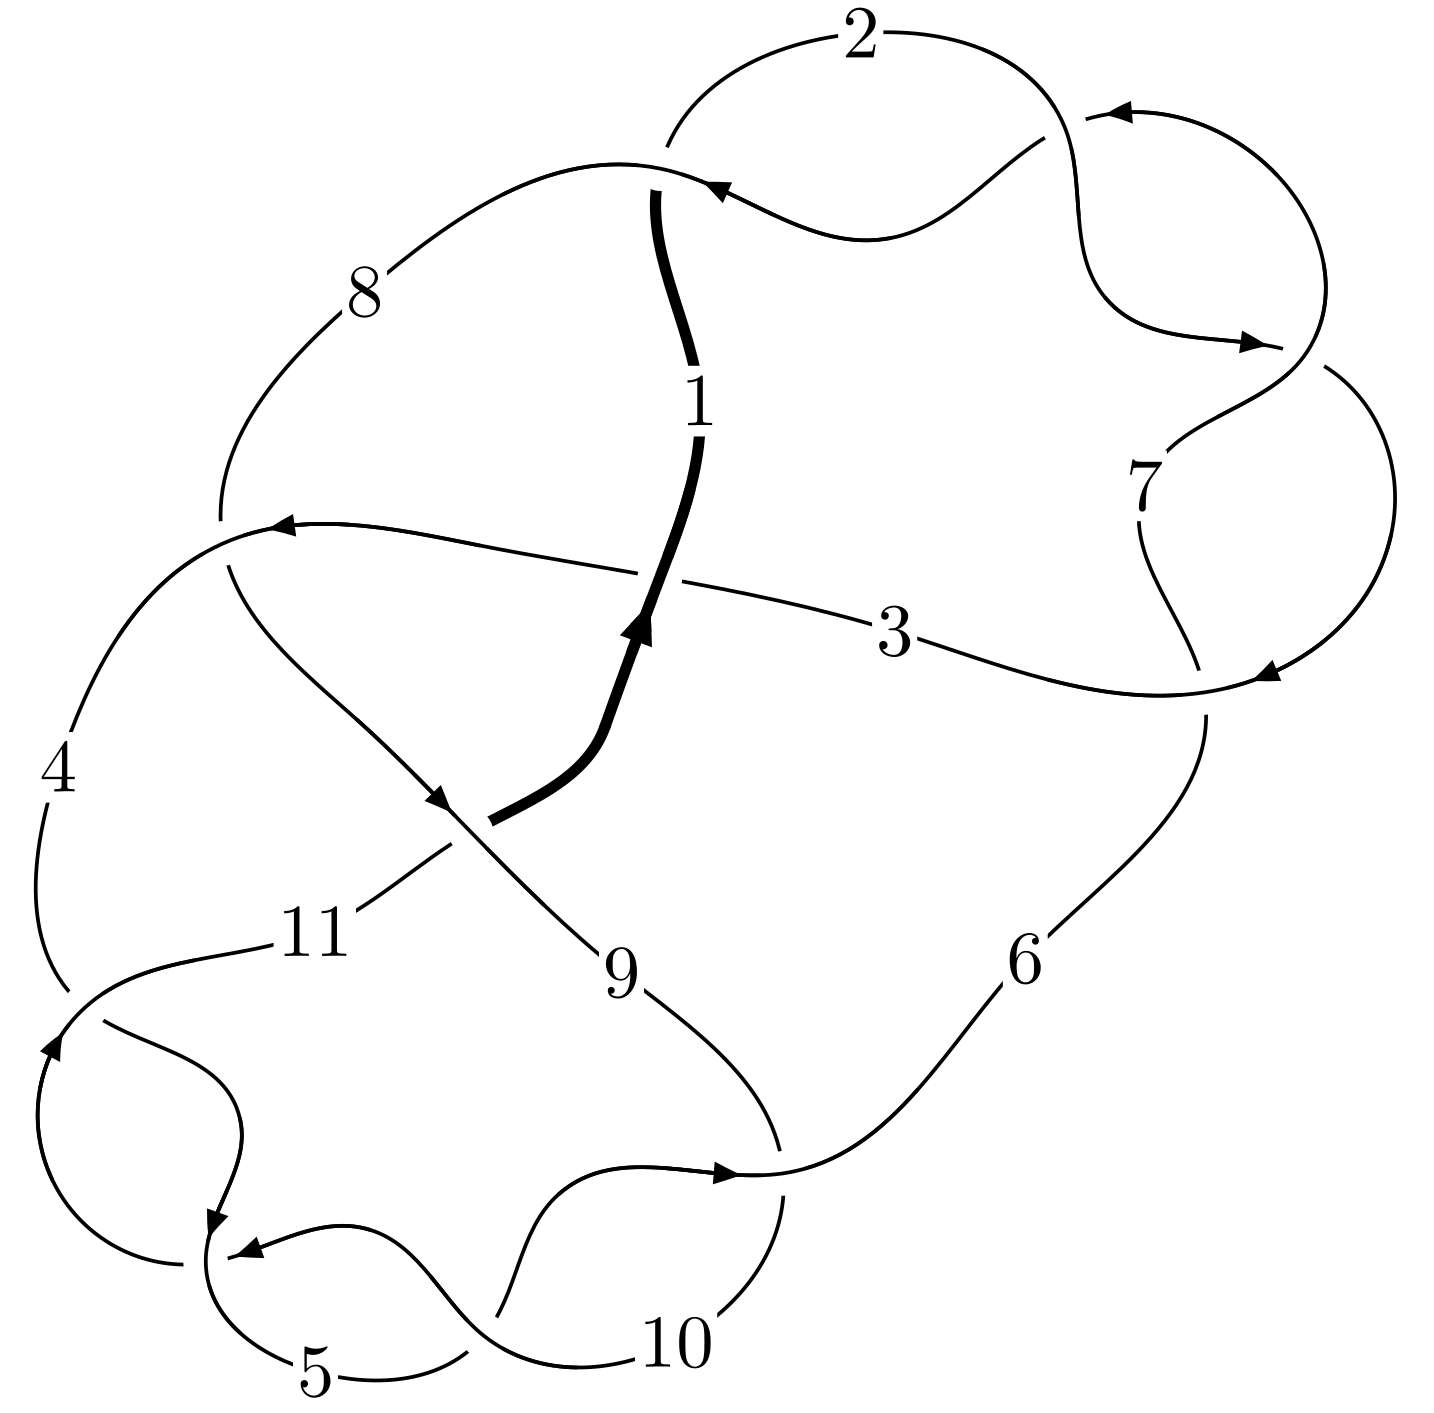
\includegraphics[width=112pt]{../../../GIT/diagram.site/Diagrams/png/582_11a_333.png}\\
\ \ \ A knot diagram\footnotemark}&
\allowdisplaybreaks
\textbf{Linearized knot diagam} \\
\cline{2-2}
 &
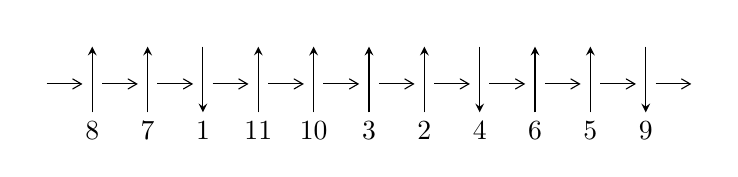
\begin{tikzpicture}[x=20pt, y=17pt]
	% nodes
	\node (C0) at (0, 0) {};
	\node (C1) at (1, 0) {};
	\node (C1U) at (1, +1) {};
	\node (C1D) at (1, -1) {8};

	\node (C2) at (2, 0) {};
	\node (C2U) at (2, +1) {};
	\node (C2D) at (2, -1) {7};

	\node (C3) at (3, 0) {};
	\node (C3U) at (3, +1) {};
	\node (C3D) at (3, -1) {1};

	\node (C4) at (4, 0) {};
	\node (C4U) at (4, +1) {};
	\node (C4D) at (4, -1) {11};

	\node (C5) at (5, 0) {};
	\node (C5U) at (5, +1) {};
	\node (C5D) at (5, -1) {10};

	\node (C6) at (6, 0) {};
	\node (C6U) at (6, +1) {};
	\node (C6D) at (6, -1) {3};

	\node (C7) at (7, 0) {};
	\node (C7U) at (7, +1) {};
	\node (C7D) at (7, -1) {2};

	\node (C8) at (8, 0) {};
	\node (C8U) at (8, +1) {};
	\node (C8D) at (8, -1) {4};

	\node (C9) at (9, 0) {};
	\node (C9U) at (9, +1) {};
	\node (C9D) at (9, -1) {6};

	\node (C10) at (10, 0) {};
	\node (C10U) at (10, +1) {};
	\node (C10D) at (10, -1) {5};

	\node (C11) at (11, 0) {};
	\node (C11U) at (11, +1) {};
	\node (C11D) at (11, -1) {9};
	\node (C12) at (12, 0) {};

	% arrows
	\draw[->,>={angle 60}]
	(C0) edge (C1) (C1) edge (C2) (C2) edge (C3) (C3) edge (C4) (C4) edge (C5) (C5) edge (C6) (C6) edge (C7) (C7) edge (C8) (C8) edge (C9) (C9) edge (C10) (C10) edge (C11) (C11) edge (C12) ;	\draw[->,>=stealth]
	(C1D) edge (C1U) (C2D) edge (C2U) (C3U) edge (C3D) (C4D) edge (C4U) (C5D) edge (C5U) (C6D) edge (C6U) (C7D) edge (C7U) (C8U) edge (C8D) (C9D) edge (C9U) (C10D) edge (C10U) (C11U) edge (C11D) ;
	\end{tikzpicture} \\
\hhline{~~} \\& 
\textbf{Solving Sequence} \\ \cline{2-2} 
 &
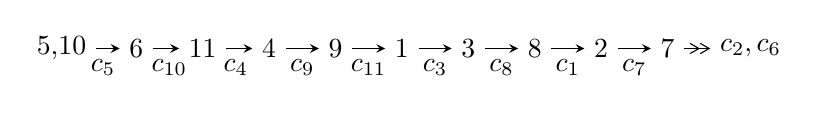
\begin{tikzpicture}[x=24pt, y=7pt]
	% node
	\node (A0) at (-1/8, 0) {5,10};
	\node (A1) at (1, 0) {6};
	\node (A2) at (2, 0) {11};
	\node (A3) at (3, 0) {4};
	\node (A4) at (4, 0) {9};
	\node (A5) at (5, 0) {1};
	\node (A6) at (6, 0) {3};
	\node (A7) at (7, 0) {8};
	\node (A8) at (8, 0) {2};
	\node (A9) at (9, 0) {7};
	\node (C1) at (1/2, -1) {$c_{5}$};
	\node (C2) at (3/2, -1) {$c_{10}$};
	\node (C3) at (5/2, -1) {$c_{4}$};
	\node (C4) at (7/2, -1) {$c_{9}$};
	\node (C5) at (9/2, -1) {$c_{11}$};
	\node (C6) at (11/2, -1) {$c_{3}$};
	\node (C7) at (13/2, -1) {$c_{8}$};
	\node (C8) at (15/2, -1) {$c_{1}$};
	\node (C9) at (17/2, -1) {$c_{7}$};
	\node (A10) at (41/4, 0) {$c_{2},c_{6}$};

	% edge
	\draw[->,>=stealth]	
	(A0) edge (A1) (A1) edge (A2) (A2) edge (A3) (A3) edge (A4) (A4) edge (A5) (A5) edge (A6) (A6) edge (A7) (A7) edge (A8) (A8) edge (A9) ;
	\draw[->>,>={angle 60}]	
	(A9) edge (A10);
\end{tikzpicture} \\ 

\end{tabular} \\

\footnotetext{
The image of knot diagram is generated by the software ``\textbf{Draw programme}" developed by Andrew Bartholomew(\url{http://www.layer8.co.uk/maths/draw/index.htm\#Running-draw}), where we modified some parts for our purpose(\url{https://github.com/CATsTAILs/LinksPainter}).
}\phantom \\ \newline 
\centering \textbf{Ideals for irreducible components\footnotemark of $X_{\text{par}}$} 
 
\begin{align*}
I^u_{1}&=\langle 
u^8+5 u^6+7 u^4+u^3+2 u^2+2 u+1\rangle \\
I^u_{2}&=\langle 
u^{24}+u^{23}+\cdots- u^3+1\rangle \\
\\
\end{align*}
\raggedright * 2 irreducible components of $\dim_{\mathbb{C}}=0$, with total 32 representations.\\
\footnotetext{All coefficients of polynomials are rational numbers. But the coefficients are sometimes approximated in decimal forms when there is not enough margin.}
\newpage
\renewcommand{\arraystretch}{1}
\centering \section*{I. $I^u_{1}= \langle u^8+5 u^6+7 u^4+u^3+2 u^2+2 u+1 \rangle$}
\flushleft \textbf{(i) Arc colorings}\\
\begin{tabular}{m{7pt} m{180pt} m{7pt} m{180pt} }
\flushright $a_{5}=$&$\begin{pmatrix}1\\0\end{pmatrix}$ \\
\flushright $a_{10}=$&$\begin{pmatrix}0\\u\end{pmatrix}$ \\
\flushright $a_{6}=$&$\begin{pmatrix}1\\- u^2\end{pmatrix}$ \\
\flushright $a_{11}=$&$\begin{pmatrix}u\\u\end{pmatrix}$ \\
\flushright $a_{4}=$&$\begin{pmatrix}u^2+1\\u^2\end{pmatrix}$ \\
\flushright $a_{9}=$&$\begin{pmatrix}- u\\u^3+u\end{pmatrix}$ \\
\flushright $a_{1}=$&$\begin{pmatrix}- u^5-2 u^3+u\\u^7+3 u^5+2 u^3+u\end{pmatrix}$ \\
\flushright $a_{3}=$&$\begin{pmatrix}u^7+4 u^5+u^4+4 u^3+3 u^2+u+1\\u^7- u^6+3 u^5-2 u^4+u^3+u^2\end{pmatrix}$ \\
\flushright $a_{8}=$&$\begin{pmatrix}u^7+4 u^5+4 u^3\\u^7+3 u^5+2 u^3+u\end{pmatrix}$ \\
\flushright $a_{2}=$&$\begin{pmatrix}- u^6- u^5-3 u^4-3 u^3-2 u^2- u-1\\u^7-2 u^6+3 u^5-5 u^4+u^3- u^2- u-1\end{pmatrix}$ \\
\flushright $a_{7}=$&$\begin{pmatrix}- u^6+u^5-3 u^4+2 u^3- u^2- u\\- u^7-2 u^6-2 u^5-6 u^4-3 u^2-2 u-1\end{pmatrix}$\\ \flushright $a_{7}=$&$\begin{pmatrix}- u^6+u^5-3 u^4+2 u^3- u^2- u\\- u^7-2 u^6-2 u^5-6 u^4-3 u^2-2 u-1\end{pmatrix}$\\&\end{tabular}
\flushleft \textbf{(ii) Obstruction class $= -1$}\\~\\
\flushleft \textbf{(iii) Cusp Shapes $= 4 u^7-4 u^6+20 u^5-16 u^4+24 u^3-12 u^2-4 u+6$}\\~\\
\newpage\renewcommand{\arraystretch}{1}
\flushleft \textbf{(iv) u-Polynomials at the component}\newline \\
\begin{tabular}{m{50pt}|m{274pt}}
Crossings & \hspace{64pt}u-Polynomials at each crossing \\
\hline $$\begin{aligned}c_{1},c_{2},c_{4}\\c_{5},c_{6},c_{7}\\c_{9},c_{10}\end{aligned}$$&$\begin{aligned}
&u^8+5 u^6+7 u^4- u^3+2 u^2-2 u+1
\end{aligned}$\\
\hline $$\begin{aligned}c_{3},c_{11}\end{aligned}$$&$\begin{aligned}
&u^8-2 u^7+3 u^6+5 u^4-5 u^3+6 u^2-2 u+1
\end{aligned}$\\
\hline $$\begin{aligned}c_{8}\end{aligned}$$&$\begin{aligned}
&u^8-5 u^7+11 u^6-16 u^5+22 u^4-27 u^3+23 u^2-12 u+4
\end{aligned}$\\
\hline
\end{tabular}\\~\\
\newpage\renewcommand{\arraystretch}{1}
\flushleft \textbf{(v) Riley Polynomials at the component}\newline \\
\begin{tabular}{m{50pt}|m{274pt}}
Crossings & \hspace{64pt}Riley Polynomials at each crossing \\
\hline $$\begin{aligned}c_{1},c_{2},c_{4}\\c_{5},c_{6},c_{7}\\c_{9},c_{10}\end{aligned}$$&$\begin{aligned}
&y^8+10 y^7+39 y^6+74 y^5+71 y^4+37 y^3+14 y^2+1
\end{aligned}$\\
\hline $$\begin{aligned}c_{3},c_{11}\end{aligned}$$&$\begin{aligned}
&y^8+2 y^7+19 y^6+22 y^5+55 y^4+41 y^3+26 y^2+8 y+1
\end{aligned}$\\
\hline $$\begin{aligned}c_{8}\end{aligned}$$&$\begin{aligned}
&y^8-3 y^7+5 y^6+4 y^5+14 y^4-13 y^3+57 y^2+40 y+16
\end{aligned}$\\
\hline
\end{tabular}\\~\\
\newpage\flushleft \textbf{(vi) Complex Volumes and Cusp Shapes}
$$\begin{array}{c|c|c}  
\text{Solutions to }I^u_{1}& \I (\text{vol} + \sqrt{-1}CS) & \text{Cusp shape}\\
 \hline 
\begin{aligned}
u &= \phantom{-}0.461135 + 0.691908 I\end{aligned}
 & -1.71296 + 5.69915 I & \phantom{-}0.47037 - 9.01967 I \\ \hline\begin{aligned}
u &= \phantom{-}0.461135 - 0.691908 I\end{aligned}
 & -1.71296 - 5.69915 I & \phantom{-}0.47037 + 9.01967 I \\ \hline\begin{aligned}
u &= \phantom{-}0.08626 + 1.49661 I\end{aligned}
 & -11.28300 + 3.64910 I & -1.10964 - 3.07905 I \\ \hline\begin{aligned}
u &= \phantom{-}0.08626 - 1.49661 I\end{aligned}
 & -11.28300 - 3.64910 I & -1.10964 + 3.07905 I \\ \hline\begin{aligned}
u &= -0.404853 + 0.285137 I\end{aligned}
 & \phantom{-}0.853870 - 0.627235 I & \phantom{-}8.80552 + 5.03557 I \\ \hline\begin{aligned}
u &= -0.404853 - 0.285137 I\end{aligned}
 & \phantom{-}0.853870 + 0.627235 I & \phantom{-}8.80552 - 5.03557 I \\ \hline\begin{aligned}
u &= -0.14255 + 1.61382 I\end{aligned}
 & -17.4667 - 10.2751 I & -4.16626 + 5.30618 I \\ \hline\begin{aligned}
u &= -0.14255 - 1.61382 I\end{aligned}
 & -17.4667 + 10.2751 I & -4.16626 - 5.30618 I\\
 \hline 
 \end{array}$$\newpage\newpage\renewcommand{\arraystretch}{1}
\centering \section*{II. $I^u_{2}= \langle u^{24}+u^{23}+\cdots- u^3+1 \rangle$}
\flushleft \textbf{(i) Arc colorings}\\
\begin{tabular}{m{7pt} m{180pt} m{7pt} m{180pt} }
\flushright $a_{5}=$&$\begin{pmatrix}1\\0\end{pmatrix}$ \\
\flushright $a_{10}=$&$\begin{pmatrix}0\\u\end{pmatrix}$ \\
\flushright $a_{6}=$&$\begin{pmatrix}1\\- u^2\end{pmatrix}$ \\
\flushright $a_{11}=$&$\begin{pmatrix}u\\u\end{pmatrix}$ \\
\flushright $a_{4}=$&$\begin{pmatrix}u^2+1\\u^2\end{pmatrix}$ \\
\flushright $a_{9}=$&$\begin{pmatrix}- u\\u^3+u\end{pmatrix}$ \\
\flushright $a_{1}=$&$\begin{pmatrix}- u^5-2 u^3+u\\u^7+3 u^5+2 u^3+u\end{pmatrix}$ \\
\flushright $a_{3}=$&$\begin{pmatrix}u^{14}+7 u^{12}+16 u^{10}+11 u^8-2 u^6+1\\- u^{16}-8 u^{14}-24 u^{12}-34 u^{10}-26 u^8-14 u^6-4 u^4\end{pmatrix}$ \\
\flushright $a_{8}=$&$\begin{pmatrix}u^7+4 u^5+4 u^3\\u^7+3 u^5+2 u^3+u\end{pmatrix}$ \\
\flushright $a_{2}=$&$\begin{pmatrix}u^{21}+12 u^{19}+\cdots-2 u^3+u\\u^{21}+11 u^{19}+\cdots+u^3+u\end{pmatrix}$ \\
\flushright $a_{7}=$&$\begin{pmatrix}2 u^{23}+u^{22}+\cdots+u+2\\- u^{22}-12 u^{20}+\cdots-2 u^3+u^2\end{pmatrix}$\\ \flushright $a_{7}=$&$\begin{pmatrix}2 u^{23}+u^{22}+\cdots+u+2\\- u^{22}-12 u^{20}+\cdots-2 u^3+u^2\end{pmatrix}$\\&\end{tabular}
\flushleft \textbf{(ii) Obstruction class $= -1$}\\~\\
\flushleft \textbf{(iii) Cusp Shapes $= 4 u^{23}+52 u^{21}+276 u^{19}-4 u^{18}+760 u^{17}-40 u^{16}+1136 u^{15}-148 u^{14}+880 u^{13}-232 u^{12}+328 u^{11}-96 u^{10}+84 u^9+92 u^8+4 u^7+64 u^6-4 u^5+16 u^4+4 u^3-4 u^2+8 u+2$}\\~\\
\newpage\renewcommand{\arraystretch}{1}
\flushleft \textbf{(iv) u-Polynomials at the component}\newline \\
\begin{tabular}{m{50pt}|m{274pt}}
Crossings & \hspace{64pt}u-Polynomials at each crossing \\
\hline $$\begin{aligned}c_{1},c_{2},c_{4}\\c_{5},c_{6},c_{7}\\c_{9},c_{10}\end{aligned}$$&$\begin{aligned}
&u^{24}- u^{23}+\cdots+u^3+1
\end{aligned}$\\
\hline $$\begin{aligned}c_{3},c_{11}\end{aligned}$$&$\begin{aligned}
&u^{24}-7 u^{23}+\cdots-94 u+17
\end{aligned}$\\
\hline $$\begin{aligned}c_{8}\end{aligned}$$&$\begin{aligned}
&(u^{12}+2 u^{11}+\cdots+2 u+3)^{2}
\end{aligned}$\\
\hline
\end{tabular}\\~\\
\newpage\renewcommand{\arraystretch}{1}
\flushleft \textbf{(v) Riley Polynomials at the component}\newline \\
\begin{tabular}{m{50pt}|m{274pt}}
Crossings & \hspace{64pt}Riley Polynomials at each crossing \\
\hline $$\begin{aligned}c_{1},c_{2},c_{4}\\c_{5},c_{6},c_{7}\\c_{9},c_{10}\end{aligned}$$&$\begin{aligned}
&y^{24}+27 y^{23}+\cdots-2 y^2+1
\end{aligned}$\\
\hline $$\begin{aligned}c_{3},c_{11}\end{aligned}$$&$\begin{aligned}
&y^{24}-9 y^{23}+\cdots-2376 y+289
\end{aligned}$\\
\hline $$\begin{aligned}c_{8}\end{aligned}$$&$\begin{aligned}
&(y^{12}-6 y^{11}+\cdots-46 y+9)^{2}
\end{aligned}$\\
\hline
\end{tabular}\\~\\
\newpage\flushleft \textbf{(vi) Complex Volumes and Cusp Shapes}
$$\begin{array}{c|c|c}  
\text{Solutions to }I^u_{2}& \I (\text{vol} + \sqrt{-1}CS) & \text{Cusp shape}\\
 \hline 
\begin{aligned}
u &= -0.288696 + 0.833188 I\end{aligned}
 & -10.86470 + 1.36952 I & -4.42656 + 0.88523 I \\ \hline\begin{aligned}
u &= -0.288696 - 0.833188 I\end{aligned}
 & -10.86470 - 1.36952 I & -4.42656 - 0.88523 I \\ \hline\begin{aligned}
u &= -0.489583 + 0.725679 I\end{aligned}
 & -9.51380 - 7.90456 I & -1.91927 + 6.92574 I \\ \hline\begin{aligned}
u &= -0.489583 - 0.725679 I\end{aligned}
 & -9.51380 + 7.90456 I & -1.91927 - 6.92574 I \\ \hline\begin{aligned}
u &= \phantom{-}0.271534 + 0.725672 I\end{aligned}
 & -2.90121\phantom{ +0.000000I} & -3.57147 + 0. I\phantom{ +0.000000I} \\ \hline\begin{aligned}
u &= \phantom{-}0.271534 - 0.725672 I\end{aligned}
 & -2.90121\phantom{ +0.000000I} & -3.57147 + 0. I\phantom{ +0.000000I} \\ \hline\begin{aligned}
u &= -0.409437 + 0.638189 I\end{aligned}
 & -0.18849 - 2.30634 I & \phantom{-}4.56865 + 4.07548 I \\ \hline\begin{aligned}
u &= -0.409437 - 0.638189 I\end{aligned}
 & -0.18849 + 2.30634 I & \phantom{-}4.56865 - 4.07548 I \\ \hline\begin{aligned}
u &= \phantom{-}0.493302 + 0.448019 I\end{aligned}
 & -4.94432 + 1.72225 I & \phantom{-}2.81956 - 4.07903 I \\ \hline\begin{aligned}
u &= \phantom{-}0.493302 - 0.448019 I\end{aligned}
 & -4.94432 - 1.72225 I & \phantom{-}2.81956 + 4.07903 I \\ \hline\begin{aligned}
u &= -0.591891 + 0.137722 I\end{aligned}
 & -7.79349 + 4.22631 I & \phantom{-}1.67942 - 2.13120 I \\ \hline\begin{aligned}
u &= -0.591891 - 0.137722 I\end{aligned}
 & -7.79349 - 4.22631 I & \phantom{-}1.67942 + 2.13120 I \\ \hline\begin{aligned}
u &= \phantom{-}0.516875 + 0.160721 I\end{aligned}
 & -0.18849 - 2.30634 I & \phantom{-}4.56865 + 4.07548 I \\ \hline\begin{aligned}
u &= \phantom{-}0.516875 - 0.160721 I\end{aligned}
 & -0.18849 + 2.30634 I & \phantom{-}4.56865 - 4.07548 I \\ \hline\begin{aligned}
u &= -0.02617 + 1.49212 I\end{aligned}
 & -4.94432 - 1.72225 I & \phantom{-}2.81956 + 4.07903 I \\ \hline\begin{aligned}
u &= -0.02617 - 1.49212 I\end{aligned}
 & -4.94432 + 1.72225 I & \phantom{-}2.81956 - 4.07903 I \\ \hline\begin{aligned}
u &= -0.11519 + 1.59101 I\end{aligned}
 & -7.79349 - 4.22631 I & \phantom{-}1.67942 + 2.13120 I \\ \hline\begin{aligned}
u &= -0.11519 - 1.59101 I\end{aligned}
 & -7.79349 + 4.22631 I & \phantom{-}1.67942 - 2.13120 I \\ \hline\begin{aligned}
u &= \phantom{-}0.08387 + 1.60577 I\end{aligned}
 & -10.86470 + 1.36952 I & -4.42656 + 0.88523 I \\ \hline\begin{aligned}
u &= \phantom{-}0.08387 - 1.60577 I\end{aligned}
 & -10.86470 - 1.36952 I & -4.42656 - 0.88523 I \\ \hline\begin{aligned}
u &= \phantom{-}0.13255 + 1.60291 I\end{aligned}
 & -9.51380 + 7.90456 I & -1.91927 - 6.92574 I \\ \hline\begin{aligned}
u &= \phantom{-}0.13255 - 1.60291 I\end{aligned}
 & -9.51380 - 7.90456 I & -1.91927 + 6.92574 I \\ \hline\begin{aligned}
u &= -0.07716 + 1.63217 I\end{aligned}
 & -19.3156\phantom{ +0.000000I} & -5.87212 + 0. I\phantom{ +0.000000I} \\ \hline\begin{aligned}
u &= -0.07716 - 1.63217 I\end{aligned}
 & -19.3156\phantom{ +0.000000I} & -5.87212 + 0. I\phantom{ +0.000000I}\\
 \hline 
 \end{array}$$\newpage
\newpage\renewcommand{\arraystretch}{1}
\centering \section*{ III. u-Polynomials}
\begin{tabular}{m{50pt}|m{274pt}}
Crossings & \hspace{64pt}u-Polynomials at each crossing \\
\hline $$\begin{aligned}c_{1},c_{2},c_{4}\\c_{5},c_{6},c_{7}\\c_{9},c_{10}\end{aligned}$$&$\begin{aligned}
&(u^8+5 u^6+7 u^4- u^3+2 u^2-2 u+1)(u^{24}- u^{23}+\cdots+u^3+1)
\end{aligned}$\\
\hline $$\begin{aligned}c_{3},c_{11}\end{aligned}$$&$\begin{aligned}
&(u^8-2 u^7+3 u^6+5 u^4-5 u^3+6 u^2-2 u+1)\\
&\cdot(u^{24}-7 u^{23}+\cdots-94 u+17)
\end{aligned}$\\
\hline $$\begin{aligned}c_{8}\end{aligned}$$&$\begin{aligned}
&(u^8-5 u^7+11 u^6-16 u^5+22 u^4-27 u^3+23 u^2-12 u+4)\\
&\cdot(u^{12}+2 u^{11}+\cdots+2 u+3)^{2}
\end{aligned}$\\
\hline
\end{tabular}\newpage\renewcommand{\arraystretch}{1}
\centering \section*{ IV. Riley Polynomials}
\begin{tabular}{m{50pt}|m{274pt}}
Crossings & \hspace{64pt}Riley Polynomials at each crossing \\
\hline $$\begin{aligned}c_{1},c_{2},c_{4}\\c_{5},c_{6},c_{7}\\c_{9},c_{10}\end{aligned}$$&$\begin{aligned}
&(y^8+10 y^7+39 y^6+74 y^5+71 y^4+37 y^3+14 y^2+1)\\
&\cdot(y^{24}+27 y^{23}+\cdots-2 y^2+1)
\end{aligned}$\\
\hline $$\begin{aligned}c_{3},c_{11}\end{aligned}$$&$\begin{aligned}
&(y^8+2 y^7+19 y^6+22 y^5+55 y^4+41 y^3+26 y^2+8 y+1)\\
&\cdot(y^{24}-9 y^{23}+\cdots-2376 y+289)
\end{aligned}$\\
\hline $$\begin{aligned}c_{8}\end{aligned}$$&$\begin{aligned}
&(y^8-3 y^7+5 y^6+4 y^5+14 y^4-13 y^3+57 y^2+40 y+16)\\
&\cdot(y^{12}-6 y^{11}+\cdots-46 y+9)^{2}
\end{aligned}$\\
\hline
\end{tabular}
\vskip 2pc
\end{document}